\documentclass{article}
\usepackage[backend=biber,natbib=true,style=alphabetic,maxbibnames=50]{biblatex}
\addbibresource{/home/nqbh/reference/bib.bib}
\usepackage[utf8]{vietnam}
\usepackage{tocloft}
\renewcommand{\cftsecleader}{\cftdotfill{\cftdotsep}}
\usepackage[colorlinks=true,linkcolor=blue,urlcolor=red,citecolor=magenta]{hyperref}
\usepackage{amsmath,amssymb,amsthm,enumitem,float,graphicx,mathtools,tikz}
\usetikzlibrary{angles,calc,intersections,matrix,patterns,quotes,shadings}
\allowdisplaybreaks
\newtheorem{assumption}{Assumption}
\newtheorem{baitoan}{}
\newtheorem{cauhoi}{Câu hỏi}
\newtheorem{conjecture}{Conjecture}
\newtheorem{corollary}{Corollary}
\newtheorem{dangtoan}{Dạng toán}
\newtheorem{definition}{Definition}
\newtheorem{dinhly}{Định lý}
\newtheorem{dinhnghia}{Định nghĩa}
\newtheorem{example}{Example}
\newtheorem{ghichu}{Ghi chú}
\newtheorem{hequa}{Hệ quả}
\newtheorem{hypothesis}{Hypothesis}
\newtheorem{lemma}{Lemma}
\newtheorem{luuy}{Lưu ý}
\newtheorem{nhanxet}{Nhận xét}
\newtheorem{notation}{Notation}
\newtheorem{note}{Note}
\newtheorem{principle}{Principle}
\newtheorem{problem}{Problem}
\newtheorem{proposition}{Proposition}
\newtheorem{question}{Question}
\newtheorem{remark}{Remark}
\newtheorem{theorem}{Theorem}
\newtheorem{vidu}{Ví dụ}
\usepackage[left=1cm,right=1cm,top=5mm,bottom=5mm,footskip=4mm]{geometry}
\def\labelitemii{$\circ$}
\DeclareRobustCommand{\divby}{%
	\mathrel{\vbox{\baselineskip.65ex\lineskiplimit0pt\hbox{.}\hbox{.}\hbox{.}}}%
}
\def\labelitemii{$\circ$}
\setlist[itemize]{leftmargin=*}
\setlist[enumerate]{leftmargin=*}

\title{Problem: Trigonometry In Triangles\\Bài Tập: Hệ Thức Lượng Trong Tam Giác}
\author{Nguyễn Quản Bá Hồng\footnote{A Scientist {\it\&} Creative Artist Wannabe. E-mail: {\tt nguyenquanbahong@gmail.com}. Bến Tre City, Việt Nam.}}
\date{\today}

\begin{document}
\maketitle
\begin{abstract}
	This text is a part of the series {\it Some Topics in Elementary STEM \& Beyond}:
	
	{\sc url}: \url{https://nqbh.github.io/elementary_STEM}.
	
	Latest version:
	\begin{itemize}
		\item {\it Problem: Trigonometry In Triangles -- Bài Tập: Hệ Thức Lượng Trong Tam Giác}.
		
		PDF: {\sc url}: \url{https://github.com/NQBH/elementary_STEM_beyond/blob/main/elementary_mathematics/grade_9/trigonometry/problem/NQBH_trigonometry_problem.pdf}.
		
		\TeX: {\sc url}: \url{https://github.com/NQBH/elementary_STEM_beyond/blob/main/elementary_mathematics/grade_9/trigonometry/problem/NQBH_trigonometry_problem.tex}.
		\item {\it Problem \& Solution: Trigonometry In Triangles -- Bài Tập \& Lời Giải: Hệ Thức Lượng Trong Tam Giác}.
		
		PDF: {\sc url}: \url{https://github.com/NQBH/elementary_STEM_beyond/blob/main/elementary_mathematics/grade_9/trigonometry/solution/NQBH_trigonometry_solution.pdf}.
		
		\TeX: {\sc url}: \url{https://github.com/NQBH/elementary_STEM_beyond/blob/main/elementary_mathematics/grade_9/trigonometry/solution/NQBH_trigonometry_solution.tex}.
	\end{itemize}
\end{abstract}
\tableofcontents

%------------------------------------------------------------------------------%

\section{1 Số Hệ Thức Lượng về Cạnh \& Đường Cao Trong Tam Giác Vuông}
$\Delta ABC$ vuông tại $A$: $a\coloneqq BC$, $b\coloneqq CA$, $c\coloneqq AB$, $b'\coloneqq CH$, $c'\coloneqq BH$, $h\coloneqq AH$. \fbox{1} Trong tam giác vuông, bình phương độ dài mỗi cạnh góc vuông bằng tích độ dài cạnh huyền \& hình chiếu của cạnh góc vuông đó trên cạnh huyền: $b^2 = ab'$, $c^2 = ac'$. \fbox{2} {\it Định lý Pythagore thuận}: Trong tam giác vuông, bình phương độ dài cạnh huyền bằng tổng bình phương độ dài 2 cạnh góc vuông. {\it Định lý Pythagore đảo}: 1 tam giác là tam giác vuông nếu bình phương 1 cạnh bằng tổng bình phương 2 cạnh còn lại. $\Delta ABC$ vuông tại $A\Leftrightarrow a^2 = b^2 + c^2$. \fbox{3} Trong tam giác vuông, bình phương độ dài đường cao bằng tích độ dài hình chiếu của 2 cạnh góc vuông lên cạnh huyền: $h^2 = b'c'$. \fbox{4} Trong tam giác vuông, tích độ dài 2 cạnh góc vuông bằng tích độ dài cạnh huyền với đường cao tương ứng: $ah = bc = 2S_{ABC}$. \fbox{5} Trong tam giác vuông, nghịch đảo bình phương độ dài đường cao bằng tổng nghịch đảo bình phương độ dài 2 cạnh góc vuông: $\dfrac{1}{h^2} = \dfrac{1}{b^2} + \dfrac{1}{c^2}$.

\begin{baitoan}[\cite{Son_Tinh_Trung_Nhuan_htl}, VD1, p. 11]
	Cho $\Delta ABC$ vuông tại A. Kẻ phân giác CD, kẻ $AH\bot CD$ tại H. Tính $AD,CD,AH$ theo $a,b,c$.
\end{baitoan}

\begin{baitoan}[\cite{Tuyen_Toan_9_old}, Thí dụ 1, p. 103]
	Cho hình thang $ABCD$ có $\widehat{B} = \widehat{C} = 90^\circ$, 2 đường chéo vuông góc với nhau tại $H$. Biết $AB = 3\sqrt{5}$ \emph{cm}, $HA = 3$ \emph{cm}. Chứng minh: (a) $HA:HB:HC:HD = 1:2:4:8$. (b) $\dfrac{1}{AB^2} - \dfrac{1}{CD^2} = \dfrac{1}{HB^2} - \dfrac{1}{HC^2}$. (c) Tính $AD,CD$.
\end{baitoan}

\begin{baitoan}[\cite{Tuyen_Toan_9_old}, 1., p. 105]
	Cho hình thang $ABCD$, $AB\parallel CD$, 2 đường chéo vuông góc với nhau. Biết $AC = 16$ \emph{cm}, $BD = 12$ \emph{cm}. Tính chiều cao của hình thang.
\end{baitoan}

\begin{baitoan}[\cite{Tuyen_Toan_9_old}, 2., p. 105]
	Cho $\Delta ABC$ vuông tại $A$, đường cao $AH$, đường phân giác $AD$. Biết $BH = 63$ \emph{cm}, $CH = 112$ \emph{cm}, tính $HD$.
\end{baitoan}

\begin{baitoan}[\cite{Tuyen_Toan_9_old}, 3., p. 105]
	Cho $\Delta ABC$ vuông tại $A$. 2 đường trung tuyến $AD,BE$ vuông góc với nhau tại $G$. Biết $AB = \sqrt{6}$ \emph{cm}. Tính cạnh huyền $BC$.
\end{baitoan}

\begin{baitoan}[\cite{Tuyen_Toan_9_old}, 4., p. 105]
	Gọi $a,b,c$ là các cạnh của 1 tam giác vuông, $h$ là đường cao ứng với cạnh huyền $a$. Chứng minh tam giác có các cạnh $a + h,b + c$, \& $h$ cũng là 1 tam giác vuông.
\end{baitoan}

\begin{baitoan}[\cite{Tuyen_Toan_9_old}, 5., p. 105]
	Cho $\Delta ABC$ vuông tại $A$, đường cao $AH$. Gọi $I,K$ thứ tự là hình chiếu của $H$ trên $AB,AC$. Đặt $c = AB$, $b = AC$. (a) Tính $AI,AK$ theo $b,c$. (b) Chứng minh $\dfrac{BI}{CK} = \dfrac{c^3}{b^3}$.
\end{baitoan}

\begin{baitoan}[\cite{Tuyen_Toan_9_old}, 6., p. 105]
	Cho $\Delta ABC$, $AB = 1$, $\widehat{A} = 105^\circ$, $\widehat{B} = 60^\circ$. Trên cạnh $BC$ lấy điểm $E$ sao cho $BE = 1$. Vẽ $ED\parallel AB$, $D\in AC$. Chứng minh: $\dfrac{1}{AC^2} + \dfrac{1}{AD^2} = \dfrac{4}{3}$.
\end{baitoan}

\begin{baitoan}[\cite{Tuyen_Toan_9_old}, 7., p. 105]
	Cho hình chữ nhật $ABCD$, $AB = 2BC$. Trên cạnh $BC$ lấy điểm $E$. Tia $AE$ cắt đường thẳng $CD$ tại $F$. Chứng minh: $\dfrac{1}{AB^2} = \dfrac{1}{AE^2} + \dfrac{1}{4AF^2}$.
\end{baitoan}

\begin{baitoan}[\cite{Tuyen_Toan_9_old}, 8., p. 105]
	Cho 3 đoạn thẳng có độ dài $a,b,c$. Dựng đoạn thẳng $x$ sao cho $\dfrac{1}{x^2} = \dfrac{1}{a^2} + \dfrac{1}{b^2} + \dfrac{1}{c^2}$.
\end{baitoan}

\begin{baitoan}[\cite{Tuyen_Toan_9_old}, 9., p. 105]
	Cho hình thoi $ABCD$ có $\widehat{A} = 120^\circ$. 1 đường thẳng $d$ không cắt các cạnh của hình thoi. Chứng minh: tổng các bình phương hình chiếu của $4$ cạnh với $2$ lần bình phương hình chiếu của đường chéo $AC$ trên đường thẳng $d$ không phụ thuộc vào vị trí của đường thẳng $d$.
\end{baitoan}

\begin{baitoan}[\cite{Tuyen_Toan_9_old}, 10., p. 106]
	Cho $\Delta ABC$ vuông tại $A$. Từ 1 điểm $O$ ở trong tam giác ta vẽ $OD\bot BC$, $OE\bot CA$, $OF\bot AB$. Xác định vị trí của $O$ để $OD^2 + OE^2 + OF^2$ nhỏ nhất.
\end{baitoan}

\begin{baitoan}[\cite{Binh_Toan_9_tap_1}, VD1, p. 84]
	Tính diện tích hình thang $ABCD$ có đường cao bằng {\rm12 cm}, 2 đường chéo $AC,BD$ vuông góc với nhau, $BD = 15$ {\rm cm}.
\end{baitoan}

\begin{baitoan}[\cite{Binh_Toan_9_tap_1}, VD2, p. 85]
	Hình thang cân ABCD có đáy lớn $CD = 10$ {\rm cm}, đáy nhỏ bằng đường cao, đường chéo vuông góc với cạnh bên. Tính đường cao của hình thang.
\end{baitoan}

\begin{baitoan}[\cite{Binh_Toan_9_tap_1}, VD3, p. 85]
	Tính diện tích 1 tam giác vuông có chu vi {\rm72 cm}, hiệu giữa đường trung tuyến \& đường cao ứng với cạnh huyền bằng {\rm7 cm}.
\end{baitoan}

\begin{baitoan}[\cite{Binh_Toan_9_tap_1}, 1., p. 86]
	Chứng minh định lý Pythagore bằng cách đặt 2 tam giác vuông bằng nhau $\Delta ABC = \Delta DCE$:
	\begin{center}
		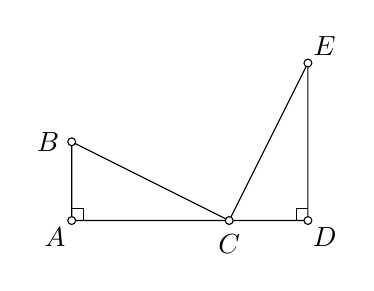
\begin{tikzpicture}
			\path
			(0,0) coordinate (A)
			(0,1) coordinate (B)
			(2,0) coordinate (C)
			(3,0) coordinate (D)
			(3,2) coordinate (E)
			;
			\draw
			(A)--(B)--(C)--cycle (C)--(D)--(E)--cycle
			pic[draw, angle radius=1.5mm]{right angle=B--A--C}
			pic[draw, angle radius=1.5mm]{right angle=C--D--E}
			;
			\foreach \x/\g in {A/-135,B/180,C/-90,D/-45,E/45} \draw[fill=white] (\x) circle (.05) + (\g:.3) node{$\x$};
		\end{tikzpicture}
	\end{center}
\end{baitoan}

\begin{baitoan}[\cite{Binh_Toan_9_tap_1}, 2., p. 86]
	Cho $\Delta ABC$ cân có $AB = AC = 9$ {\rm cm}, $BC = 12$ {\rm cm}, đường cao $AH$, I là hình chiếu của H trên AC. (a) Tính độ dài CI. (b) Kẻ đường cao BK của $\Delta ABC$. Chứng minh điểm K nằm giữa 2 điểm A, C.
\end{baitoan}

\begin{baitoan}[\cite{Binh_Toan_9_tap_1}, 3., p. 86]
	Cho $\Delta ABC$ có $\widehat{A} = 120^\circ$, $BC = a$, $AC = b$, $AB = c$. Chứng minh $a^2 = b^2 + c^2 + bc$.
\end{baitoan}

\begin{baitoan}[\cite{Binh_Toan_9_tap_1}, 4., p. 86]
	Tính cạnh đáy BC của $\Delta ABC$ cân biết đường cao ứng với cạnh đáy bằng {\rm15.6 cm} \& đường cao ứng với cạnh bên bằng {\rm12 cm}.
\end{baitoan}

\begin{baitoan}[\cite{Binh_Toan_9_tap_1}, 5., p. 86]
	Cho $\Delta ABC$ vuông tại A, đường phân giác AD, đường cao AH. Biết $BD = 7.5$ {\rm cm}, $CD = 10$ {\rm cm}. Tính AH, BH, DH.
\end{baitoan}

\begin{baitoan}[\cite{Binh_Toan_9_tap_1}, 6., p. 86]
	Cho $\Delta ABC$ vuông tại A, đường cao AH, $AB = 20$ {\rm cm}, $CH = 9$ {\rm cm}. Tính độ dài AH.
\end{baitoan}

\begin{baitoan}[\cite{Binh_Toan_9_tap_1}, 7., p. 86]
	Cho $\Delta ABC$ vuông tại A, đường cao AH. Tia phân giác của $\widehat{HAC}$ cắt HC ở D. Gọi K là hình chiếu của D trên AC. Biết $BC = 25$ {\rm cm}, $DK = 6$ {\rm cm}. Tính AB.
\end{baitoan}

\begin{baitoan}[\cite{Binh_Toan_9_tap_1}, 8., p. 86]
	Cho $\Delta ABC$ có $AB = 6$ {\rm cm}, $AC = 8$ {\rm cm}, 2 đường trung tuyến BD, CE vuông góc với nhau. Tính BC.
\end{baitoan}

\begin{baitoan}[\cite{Binh_Toan_9_tap_1}, 9., p. 86]
	Cho $\Delta ABC$ có $\widehat{B} = 60^\circ$, $BC = 8$ {\rm cm}, $AB + AC = 12$ {\rm cm}. Tính AB, AC.
\end{baitoan}

\begin{baitoan}[\cite{Binh_Toan_9_tap_1}, 10., p. 86]
	Trong 1 tam giác vuông, đường cao ứng với cạnh huyền chia tam giác thành 2 phần có diện tích bằng $\rm54\ cm^2$ \& $\rm96\ cm^2$. Tính độ dài cạnh huyền.
\end{baitoan}

\begin{baitoan}[\cite{Binh_Toan_9_tap_1}, 11., p. 86]
	Cho $\Delta ABC$ vuông cân tại A, đường trung tuyến BM. Gọi D là hình chiếu của C trên BM, H là hình chiếu của D trên AC. Chứng minh $AH = 3DH$.
\end{baitoan}

\begin{baitoan}[\cite{Binh_Toan_9_tap_1}, 12., pp. 86--87]
	(a) 1 tam giác vuông có tỷ số các cạnh góc vuông bằng $k$. Tính tỷ số các hình chiếu của 2 cạnh góc vuông trên cạnh huyền. (b) Tính độ dài hình chiếu của các cạnh góc vuông trên cạnh huyền của 1 tam giác vuông, biết tỷ số 2 cạnh góc vuông bằng $5:4$ \& cạnh huyền dài {\rm82 cm}.
\end{baitoan}

\begin{baitoan}[\cite{Binh_Toan_9_tap_1}, 13., p. 87]
	Trong 1 tam giác vuông, đường phân giác của góc vuông chia cạnh huyền thành 2 đoạn thẳng tỷ lệ với $1:3$. Đường cao ứng với cạnh huyền chia cạnh đó theo tỷ số nào?
\end{baitoan}

\begin{baitoan}[\cite{Binh_Toan_9_tap_1}, 14., p. 87]
	Cho $\Delta ABC$ có độ dài 3 cạnh AB, BC, CA là 3 số tự nhiên liên tiếp tăng dần. Kẻ đường cao AH, đường trung tuyến AM. Chứng minh $HM = 2$.
\end{baitoan}

\begin{baitoan}[\cite{Binh_Toan_9_tap_1}, 15., p. 87]
	1 hình thang cân có đường chéo vuông góc với cạnh bên. Tính chu vi \& diện tích hình thang biết đáy nhỏ dài {\rm14 cm}, đáy lớn dài {\rm50 cm}.
\end{baitoan}

\begin{baitoan}[\cite{Binh_Toan_9_tap_1}, 16., p. 87]
	1 hình thoi có diện tích bằng $\frac{1}{2}$ diện tích hình vuông có cạnh bằng cạnh của hình thoi. Tính tỷ số của đường chéo dài \& đường chéo ngắn của hình thoi.
\end{baitoan}

\begin{baitoan}[\cite{Binh_Toan_9_tap_1}, 17., p. 87]
	Qua đỉnh A của hình vuông ABCD cạnh $a$, vẽ 1 đường thẳng cắt cạnh BC ở M \& cắt đường thẳng CD ở I. Chứng minh $\dfrac{1}{AM^2} + \dfrac{1}{AI^2} = \dfrac{1}{a^2}$.
\end{baitoan}

\begin{baitoan}[\cite{Binh_Toan_9_tap_1}, 18., p. 87]
	Cho hình vuông ABCD có cạnh {\rm1 dm}. Tính cạnh của $\Delta AEF$ đều có E thuộc cạnh CD \& F thuộc cạnh BC.
\end{baitoan}

\begin{baitoan}[\cite{Binh_Toan_9_tap_1}, 19., p. 87]
	Trong 2 tam giác sau, tam giác nào là tam giác vuông, nếu độ dài 3 đường cao bằng: (a) $3,4,5$. (b) $12,15,20$.
\end{baitoan}

\begin{baitoan}[Mở rộng \cite{Binh_Toan_9_tap_1}, 19., p. 87]
	Cho tam giác ABC có 3 đường cao có độ dài lần lượt là $h_a,h_b,h_c$. Tìm điều kiện cần \& đủ theo $h_a,h_b,h_c$ để $\Delta ABC$ vuông.
\end{baitoan}

\begin{baitoan}[\cite{Binh_Toan_9_tap_1}, 20., p. 87]
	Chứng minh $\Delta ABC$ là tam giác vuông nếu 2 đường phân giác BD, CE cắt nhau tại I thỏa mãn $BD\cdot CE = 2BI\cdot CI$.
\end{baitoan}

\begin{baitoan}[\cite{Binh_Toan_9_tap_1}, 21., p. 87]
	Xét các $\Delta ABC$ vuông có cạnh huyền $BC = 2a$. Gọi AH là đường cao của tam giác, D, E lần lượt là hình chiếu của H trên AC, AB. Tìm {\rm GTLN} của: (a) DE. (b) Diện tích tứ giác $ADHE$.
\end{baitoan}

\begin{baitoan}[\cite{Binh_Toan_9_tap_1}, 22., pp. 87--88]
	Chứng minh trong 1 tam giác: (a) Bình phương của cạnh đối diện với góc nhọn bằng tổng các bình phương của 2 cạnh kia trừ đi 2 lần tích của 1 trong 2 cạnh ấy với hình chiếu của cạnh kia trên nó.
\end{baitoan}

\begin{baitoan}[\cite{Binh_Toan_9_tap_1}, 23., p. 88]
	Cho $\Delta ABC$ có $BC = a$, $CA = b$, $AB = c$. Chứng minh: (a) $b^2 < c^2 + a^2\Rightarrow\widehat{B} < 90^\circ$. (b) $b^2 > c^2 + a^2\Rightarrow\widehat{B} > 90^\circ$. (c) $b^2 = c^2 + a^2\Rightarrow\widehat{B} = 90^\circ$.
\end{baitoan}

\begin{baitoan}[\cite{Binh_Toan_9_tap_1}, 24., p. 88]
	$\Delta ABC$ vuông tại A, đường phân giác BD. Tia phân giác của $\widehat{A}$ cắt BD ở I. Biết $BI = 10\sqrt{5}$ {\rm cm}, $DI = 5\sqrt{5}$ {\rm cm}. Tính diện tích $\Delta ABC$.
\end{baitoan}

\begin{baitoan}[\cite{Binh_Toan_9_tap_1}, 25., p. 88]
	$\Delta ABC$ vuông tại A, gọi I là giao điểm của 3 đường phân giác. (a) Biết $AB = 5$ {\rm cm}, $CI = 6$ {\rm cm}. Tính BC. (b) Biết $BI = \sqrt{5}$ {\rm cm}, $CI = \sqrt{10}$ {\rm cm}. Tính AB, AC.
\end{baitoan}

\begin{baitoan}[\cite{Binh_Toan_9_tap_1}, 26., p. 88]
	Cho $\Delta ABC$ vuông tại A, gọi I là giao điểm của 3 đường phân giác, M là trung điểm của BC. (a) Biết $AB = 6$ {\rm cm}, $AC = 8$ {\rm cm}. Tính $\widehat{BIM}$. (b) Biết $\widehat{BIM} = 90^\circ$. 3 cạnh của $\Delta ABC$ tỷ lệ với 3 số nào?
\end{baitoan}

\begin{baitoan}[\cite{Binh_Toan_9_tap_1}, 27., p. 88]
	1 tam giác vuông có độ dài 1 cạnh bằng trung bình cộng của độ dài 2 cạnh kia. (a) ĐỘ dài 3 cạnh của tam giác vuông đó tỷ lệ với 3 số nào? (b) Nếu độ dài 3 cạnh của tam giác vuông đó là 3 số nguyên dương thì số nào trong 5 số sau có thể là độ dài 1 cạnh của tam giác đó: $17,13,35,41,22$?
\end{baitoan}

\begin{baitoan}[\cite{Binh_Toan_9_tap_1}, 28., p. 88]
	Cho $\Delta ABC$ vuông tại A, $BC = 3\sqrt{5}$ {\rm cm}. Hình vuông ADEF cạnh {\rm2 cm} có $D\in AB$, $E\in BC$, $F\in CA$. Tính AB, AC.
\end{baitoan}

\begin{baitoan}[\cite{Binh_Toan_9_tap_1}, 29., p. 88]
	$\Delta ABC$ cân tại A, gọi I là giao điểm của 3 đường phân giác. Biết $IA = 2\sqrt{5}$ {\rm cm}, $IB = 3$ {\rm cm}. Tính AB.
\end{baitoan}

\begin{baitoan}[\cite{Binh_Toan_9_tap_1}, 30., p. 88]
	$\Delta ABC$ cân tại A, đường cao AD, trực tâm H. Tính độ dài AD, biết $AH = 14$ {\rm cm}, $BH = CH = 30$ {\rm cm}.
\end{baitoan}

\begin{baitoan}[\cite{Binh_Toan_9_tap_1}, 31., p. 88]
	$\Delta ABC$ có $BC = 40$ {\rm cm}, đường phân giác AD dài {\rm45 cm}, đường cao AH dài {\rm36 cm}. Tính BD, CD.
\end{baitoan}

\begin{baitoan}[\cite{TLCT_THCS_Toan_9_hinh_hoc}, VD1, p. 5]
	Cho $\Delta ABC$ vuông tại $A$, đường cao $AH$. Biết $AB:AC = 3:4$ \& $AB + AC = 21$ \emph{cm}. (a) Tính các cạnh của $\Delta ABC$. (b) Tính độ dài các đoạn $AH,BH,CH$.
\end{baitoan}

\begin{baitoan}[Mở rộng \cite{TLCT_THCS_Toan_9_hinh_hoc}, VD1, p. 5]
	Cho $\Delta ABC$ vuông tại $A$, đường cao $AH$. Biết $AB:AC = m:n$ \& $AB + AC = p$ \emph{cm}. (a) Tính các cạnh của $\Delta ABC$. (b) Tính độ dài các đoạn $AH,BH,CH$.
\end{baitoan}

\begin{baitoan}[\cite{TLCT_THCS_Toan_9_hinh_hoc}, VD2, p. 6]
	Cho hình thang $ABCD$ có $\widehat{A} = \widehat{D} = 90^\circ$, $\widehat{B} = 60^\circ$, $CD = 30$ \emph{cm}, $CA\bot CB$. Tính diện tích của hình thang.
\end{baitoan}

\begin{baitoan}[\cite{TLCT_THCS_Toan_9_hinh_hoc}, VD3, p. 7]
	Cho $\Delta ABC$ nhọn, đường cao $CK$, $H$ là trực tâm. Gọi $M$ là 1 điểm trên $CK$ sao cho $\widehat{AMB} = 90^\circ$. $S,S_1,S_2$ theo thứ tự là diện tích các $\Delta AMB,\Delta ABC,\Delta ABH$. Chứng minh $S = \sqrt{S_1S_2}$.
\end{baitoan}

\begin{baitoan}[\cite{TLCT_THCS_Toan_9_hinh_hoc}, 1.1., p. 7]
	Cho $\Delta ABC$ vuông cân tại $A$ \& điểm $M$ nằm giữa $B$ \& $C$ Gọi $D,E$ lần lượt là hình chiếu của điểm $M$ lên $AB,AC$. Chứng minh $MB^2 + MC^2 = 2MA^2$.
\end{baitoan}

\begin{baitoan}[\cite{TLCT_THCS_Toan_9_hinh_hoc}, 1.2., p. 7]
	Cho hình chữ nhật $ABCD$ \& điểm $O$ nằm trong hình chữ nhật đó. Chứng minh $OA^2 + OC^2 = OB^2 + CD^2$.
\end{baitoan}

\begin{baitoan}[\cite{TLCT_THCS_Toan_9_hinh_hoc}, 1.3., p. 8]
	Cho hình chữ nhật $ABCD$ có $AD = 6$ \emph{cm}, $CD = 8$ \emph{cm}. Đường thẳng kẻ từ $D$ vuông góc với $AC$ tại $E$, cắt cạnh $AB$ tại $F$. Tính độ dài các đoạn thẳng $DE,DF,AE,CE,AF,BF$.
\end{baitoan}

\begin{baitoan}[\cite{TLCT_THCS_Toan_9_hinh_hoc}, 1.4., p. 8]
	Cho $\Delta ABC$ có $AB = 3$  \emph{cm}, $BC = 4$ \emph{cm}, $AC = 5$ \emph{cm}. Đường cao, đường phân giác, đường trung tuyến của tam giác kẻ từ đỉnh $B$ chia tam giác thành $4$ gam giác không có điểm trong chung. Tính diện tích của mỗi tam giác đó.
\end{baitoan}

\begin{baitoan}[\cite{TLCT_THCS_Toan_9_hinh_hoc}, 1.5., p. 8]
	Trong 1 tam giác vuông tỷ số giữa đường cao \& đường trung tuyến kẻ từ đỉnh góc vuông bằng $40:41$. Tính độ dài các cạnh góc vuông của tam giác đó, biết cạnh huyền bằng $\sqrt{41}$ \emph{cm}.
\end{baitoan}

\begin{baitoan}[\cite{TLCT_THCS_Toan_9_hinh_hoc}, 1.6., p. 8]
	Cho $\Delta ABC$ vuông tại $A$, đường cao $AH$. Kẻ $HE\bot AB$, $HF\bot AC$. Gọi $O$ là giao điểm của $AH$ \& $EF$. Chứng minh $HB\cdot HC = 4OE\cdot OF$.
\end{baitoan}

\begin{baitoan}[\cite{TLCT_THCS_Toan_9_hinh_hoc}, 1.7., p. 8]
	Cho $\Delta ABC$, 2 đường cao $BD,CE$ cắt nhau tại H. Gọi $M,N$ lần lượt là 2 điểm thuộc $HC,HB$ sao cho $\widehat{AMB} = \widehat{ANC} = 90^\circ$. $\Delta AMN$ là tam giác gì?
\end{baitoan}

\begin{baitoan}[\cite{TLCT_THCS_Toan_9_hinh_hoc}, 1.8., p. 8]
	Cho hình vuông ABCD, cạnh $a$. (a) M là 1 điểm trên cạnh AD sao cho $\widehat{ABM} = 30^\circ$. Tính $AM,BM$ theo $a$. (b) Qua A kẻ đường thẳng vuông góc với BM tại F, đường thẳng này cắt CD tại N. Tính độ dài 3 đoạn thẳng $AF,MF,BF$ theo $a$.
\end{baitoan}

\begin{baitoan}[\cite{TLCT_THCS_Toan_9_hinh_hoc}, 1.9., p. 8]
	Cho hình vuông ABCD \& điểm I thay đổi giữa $A,B$. Tia DI cắt BC tại E. Đường thẳng kẻ qua D vuông góc với DE cắt BC tại F. Chứng minh tổng $\dfrac{1}{DI^2} + \dfrac{1}{DE^2}$ không phụ thuộc vào vị trí của điểm I.
\end{baitoan}

\begin{baitoan}[\cite{TLCT_THCS_Toan_9_hinh_hoc}, 1.10., p. 8]
	Cho $\Delta ABC$, đường cao BH. Đặt $BC = a,CA = b,AB = c,AH = c'$. Chứng minh: (a) Nếu $\widehat{A} < 90^\circ$ thì $a^2 = b^2 + c^2 - 2bc'$. (b) Nếu $\widehat{A} > 90^\circ$ thì $a^2 = b^2 + c^2 + 2bc'$.
\end{baitoan}

\begin{baitoan}[\cite{TLCT_THCS_Toan_9_hinh_hoc}, 1.11., p. 8]
	Cho $\Delta ABC$, đường cao $AH$. Biết $AB = 8$ {\rm cm}, $BC - AC = 2$ {\rm cm}, $\widehat{BAH} = 30^\circ$. Tính diện tích $\Delta ABC$.
\end{baitoan}

\begin{baitoan}[\cite{TLCT_THCS_Toan_9_hinh_hoc}, 1.12., p. 8]
	Cho $\Delta ABC$, các đường cao ứng với các cạnh $a,b,c$ lần lượt là $h_a,h_b,h_c$. Chứng minh nếu $\frac{1}{h_a^2} = \frac{1}{h_b^2} + \frac{1}{h_c^2}$ thì $\Delta ABC$ vuông tại $A$.
\end{baitoan}

\begin{baitoan}[\cite{TLCT_THCS_Toan_9_hinh_hoc}, 1.13., p. 9]
	Cho $\Delta ABC$, 2 đường phân giác $BD,CE$ cắt nhau tại $I$ thỏa mãn $BD\cdot CE= 2BI\cdot CI$. $\Delta ABC$ là tam giác gì? Vì sao?
\end{baitoan}

\begin{baitoan}[\cite{TLCT_THCS_Toan_9_hinh_hoc}, 1.14., p. 9]
	Cho $\Delta ABC$, $\widehat{A} = 90^\circ$, $BC = 2a$, đường cao $AH$. Kẻ $HD\bot AC$, $HE\bot AB$. Tìm giá trị lớn nhất của: (a) Độ dài đoạn thẳng $DE$. (b) Diện tích tứ giác $ADHE$.
\end{baitoan}

\begin{baitoan}[\cite{TLCT_THCS_Toan_9_hinh_hoc}, 1.15., p. 9]
	Cho $\Delta ABC$ đều có cạnh bằng {\rm60 cm}. Trên đoạn $BC$ lấy điểm $D$ sao cho $BD = 20$ {\rm cm}. Đường trung trực của $AD$ cắt $AB$ tại $E$, cắt $AC$ tại $F$. Tính độ dài các cạnh của $\Delta DEF$.
\end{baitoan}

\begin{baitoan}[\cite{TLCT_THCS_Toan_9_hinh_hoc}, 1.16., p. 9]
	Cho $\Delta ABC$. Đường trung tuyến $AD$, đường cao $BH$, đường phân giác $CE$ đồng quy. Chứng minh đẳng thức $(AB + CA)(BC^2 + CA^2 - AB^2) = 2BC\cdot CA^2$ hay $(b + c)(a^2 + b^2 - c^2) = 2ab^2$.
\end{baitoan}

\begin{baitoan}[{\sf Program}: Trigonometry in right triangles]
	Cho $\Delta ABC$ vuông tại $A$. (a) {\rm(Tính độ dài cạnh, đường cao, hình chiếu trong tam giác vuông)} Cho trước 2 yếu tố trong $6 + 15 = 21$ yếu tố gồm 6 số $a,b,c,b',c',h$ \& $C_6^2 = 15$ tỷ số của chúng:
	\begin{equation*}
		\frac{a}{b},\frac{a}{c},\frac{a}{b'},\frac{a}{c'},\frac{a}{h},\frac{b}{c},\frac{b}{b'},\frac{b}{c'},\frac{b}{h},\frac{c}{b'},\frac{c}{c'},\frac{c}{h},\frac{b'}{c'},\frac{b'}{h},\frac{c'}{h}.
	\end{equation*}
	Tìm công thức của 4 số còn lại theo 2 số đã cho. (b) Cho trước 2 trong $14 + 91 = 105$ yếu tố gồm 14 số $a,b,c$, $b',c',h$, $m_a,m_b,m_c$, $d_a,d_b,d_c$, $p,S$, \& $C_{14}^2 = 91$ tỷ số của chúng, với $d_a,d_b,d_c$ lần lượt là 3 đường phân giác ứng với $BC,CA,AB$. Tính 12 số còn lại theo 2 số đã cho. Viết các chương trình {\sf Pascal, Python, C{\tt/}C++} để giải bài toán.
\end{baitoan}

%------------------------------------------------------------------------------%

\section{Tỷ Số Lượng Giác của Góc Nhọn}
\cite[Chap. IV, \S1, pp. 74--81]{SGK_Toan_9_Canh_Dieu_tap_1}: HD1. LT1. HD2. LT2. LT3. HD3. HD4. LT4. 1. 2. 3. 4. 5. 6. 7. 8.

\begin{baitoan}[\cite{Tuyen_Toan_9_old}, Thí dụ 2, p. 107]
	Cho $\cot\alpha = \dfrac{a^2 - b^2}{2ab}$ trong đó $\alpha$ là góc nhọn, $a > b > 0$. Tính $\cos\alpha$.
\end{baitoan}

\begin{baitoan}[\cite{Tuyen_Toan_9_old}, 11., p. 108, định lý sin]
	Cho $\Delta ABC$ nhọn, $BC = a$, $CA = b$, $AB = c$. Chứng minh: $\dfrac{a}{\sin A} = \dfrac{b}{\sin B} = \dfrac{c}{\sin C}$. Đẳng thức này còn đúng với tam giác vuông \& tam giác tù hay không?
\end{baitoan}

\begin{baitoan}[\cite{Tuyen_Toan_9_old}, 12., p. 108]
	Chứng minh: (a) $1 + \tan^2\alpha = \dfrac{1}{\cos^2\alpha}$. (b) $1 + \cot^2\alpha = \dfrac{1}{\sin^2\alpha}$. (c) $\cot^2\alpha - \cos^2\alpha = \cot^2\alpha\cdot\cos^2\alpha$. (d) $\dfrac{1 + \cos\alpha}{\sin\alpha} = \dfrac{\sin\alpha}{1 - \cos\alpha}$.
\end{baitoan}

\begin{baitoan}[\cite{Tuyen_Toan_9_old}, 13., p. 108]
	Rút gọn biểu thức: (a) $A = \dfrac{1 + 2\sin\alpha\cdot\cos\alpha}{\cos^2\alpha - \sin^2\alpha}$. (b) $B = (1 + \tan^2\alpha)(1 - \sin^2\alpha) - (1 + \cot^2\alpha)(1 - \cos^2\alpha)$. (c) $C = \sin^6\alpha + \cos^6\alpha + 3\sin^2\alpha\cos^2\alpha$.
\end{baitoan}

\begin{baitoan}[\cite{Tuyen_Toan_9_old}, 14., p. 108]
	Tính giá trị của biểu thức $A = 5\cos^2\alpha + 2\sin^2\alpha$ biết $\sin\alpha = \frac{2}{3}$.
\end{baitoan}

\begin{baitoan}[\cite{Tuyen_Toan_9_old}, 15., p. 108]
	Không dùng máy tính hoặc bảng số, tính: (a) $A = \cos^2 20^\circ + \cos^2 30^\circ + \cos^2 40^\circ + \cos^2 50^\circ + \cos^2 60^\circ + \cos^2 70^\circ$. (b) $B = \sin^2 5^\circ + \sin^2 25^\circ + \sin^2 45^\circ + \sin^2 65^\circ + \sin^2 85^\circ$.
\end{baitoan}

\begin{baitoan}[\cite{Tuyen_Toan_9_old}, 16., p. 108]
	Cho $0^\circ < \alpha < 90^\circ$. Chứng minh: $\sin\alpha < \tan\alpha$, $\cos\alpha < \cot\alpha$. Áp dụng: (a) Sắp xếp các số sau theo thứ tự tăng dần: $\sin 65^\circ,\cos 65^\circ,\tan 65^\circ$. (b) Xác định $\alpha$ thỏa mãn điều kiện: $\tan\alpha > \sin\alpha > \cos\alpha$.
\end{baitoan}

\begin{baitoan}[\cite{Tuyen_Toan_9_old}, 17., p. 108]
	Cho $\Delta ABC$ vuông tại $A$. Biết $\sin B = \frac{1}{4}$, tính $\tan C$.
\end{baitoan}

\begin{baitoan}[\cite{Tuyen_Toan_9_old}, 18., p. 108]
	Cho biết $\sin\alpha + \cos\alpha = \frac{7}{5}$, $0^\circ < \alpha < 90^\circ$, tính $\tan\alpha$.
\end{baitoan}

\begin{baitoan}[\cite{Tuyen_Toan_9_old}, 19., p. 109]
	$\Delta ABC$, đường trung tuyến $AM$. Chứng minh nếu $\cot B = 3\cot C$ thì $AM = AC$.
\end{baitoan}

\begin{baitoan}[\cite{Tuyen_Toan_9_old}, 20., p. 109]
	Cho $\Delta ABC$, trực tâm $H$ là trung điểm của đường cao $AD$. Chứng minh $\tan B\tan C = 2$.
\end{baitoan}

\begin{baitoan}[\cite{Tuyen_Toan_9_old}, 21., p. 109]
	Cho $\Delta ABC$ nhọn, 2 đường cao $BD,CE$. Chứng minh: (a) $S_{\Delta ADE} = S_{\Delta ABC}\cos^2A$. (b) $S_{BCDE} = S_{\Delta ABC}\sin^2A$.
\end{baitoan}

\begin{baitoan}[\cite{Tuyen_Toan_9_old}, 22., p. 109]
	Cho $\Delta ABC$ nhọn. Từ 1 điểm $M$ nằm trong tam giác vẽ $MD\bot BC$, $ME\bot AC$, $MF\bot AB$. Chứng minh $\max\{MA,MB,MC\}\ge2\min\{MD,ME,MF\}$, trong đó $\max\{MA,MB,MC\}$ là đoạn thẳng lớn nhất trong các đoạn thẳng $MA,MB,MC$ \& $\min\{MD,ME,MF\}$ là đoạn thẳng nhỏ nhất trong các đoạn thẳng $MD,ME,MF$.
\end{baitoan}

\begin{baitoan}[\cite{Binh_Toan_9_tap_1}, VD4, p. 89]
	Tính $\tan15^\circ$ mà không cần dùng bảng số, không dùng máy tính.
\end{baitoan}

\begin{baitoan}[\cite{Binh_Toan_9_tap_1}, VD4, p. 90]
	Xét $\Delta ABC$ vuông tại A, $AB < AC$, $\widehat{C} = \alpha  < 45^\circ$, đường trung tuyến AM, đường cao AH, $MA = MB = MC = a$. Chứng minh: (a) $\sin2\alpha = 2\sin\alpha\cos\alpha$. (b) $1 + \cos2\alpha = 2\cos^2\alpha$. (c) $1 - \cos2\alpha = 2\sin^2\alpha$.
\end{baitoan}

\begin{baitoan}[\cite{Binh_Toan_9_tap_1}, 32., p. 91]
	Tính sai số của 2 phép dựng: (a) Dựng góc $72^\circ$ bằng cách dựng góc nhọn của tam giác vuông có 2 cạnh góc vuông bằng {\rm1 cm} \& {\rm3 cm}. (b) Dựng góc $20^\circ$ bằng cách dựng góc ở đỉnh của tam giác cân có đáy {\rm2 cm}, cạnh bên {\rm6 cm}.
\end{baitoan}

\begin{baitoan}[\cite{Binh_Toan_9_tap_1}, 33., p. 91]
	$\Delta ABC$ có đường trung tuyến AM bằng cạnh AC. Tính $\dfrac{\tan B}{\tan C}$.
\end{baitoan}

\begin{baitoan}[\cite{Binh_Toan_9_tap_1}, 34., p. 91]
	Cho $\tan\alpha = \frac{1}{2}$. Tính $\dfrac{\cos\alpha + \sin\alpha}{\cos\alpha - \sin\alpha}$.
\end{baitoan}

\begin{baitoan}[\cite{Binh_Toan_9_tap_1}, 35., p. 91]
	Cho hình vuông ABCDN. M, N lần lượt là trung điểm của BC, CD. Tính $\cos\widehat{MAN}$.
\end{baitoan}

\begin{baitoan}[\cite{Binh_Toan_9_tap_1}, 36., p. 91]
	Cho $\Delta ABC$ vuông tại A, đường cao AH. Gọi D là điểm đối xứng với A qua B. Gọi E là điểm thuộc tia đối của tia AH sao cho $HE = 2HA$. Chứng minh $\widehat{DEC} = 90^\circ$.
\end{baitoan}

\begin{baitoan}[\cite{Binh_Toan_9_tap_1}, 37., p. 91]
	Chứng minh trong 1 tam giác, đường phân giác ứng với cạnh lớn nhất nhỏ hơn hoặc bằng đường cao ứng với cạnh nhỏ nhất.
\end{baitoan}

\begin{baitoan}[\cite{Binh_Toan_9_tap_1}, 38., p. 91]
	Tính $\tan22^\circ30'$ mà không dùng bảng số hay máy tính.
\end{baitoan}

\begin{baitoan}[\cite{Binh_Toan_9_tap_1}, 39., p. 91]
	Chứng minh $\cos15^\circ = \dfrac{\sqrt{6} + \sqrt{2}}{4}$, $\sin15^\circ = \dfrac{\sqrt{6} - \sqrt{2}}{4}$ mà không dùng bảng số hay máy tính.
\end{baitoan}

\begin{baitoan}[\cite{Binh_Toan_9_tap_1}, 40., p. 91]
	Tính $\cos36^\circ,\cos72^\circ$ mà không dùng bảng số hay máy tính.
\end{baitoan}

\begin{baitoan}[\cite{TLCT_THCS_Toan_9_hinh_hoc}, VD1, p. 10]
	Biết $\sin\alpha = \dfrac{5}{13}$. Tính $\cos\alpha,\tan\alpha,\cot\alpha$.
\end{baitoan}

\begin{baitoan}[\cite{TLCT_THCS_Toan_9_hinh_hoc}, VD2, p. 11]
	Cho $\Delta ABC$ nhọn, 2 đường cao $AD,BE$ cắt nhau tại $H$. Biết $HD:HA = 1:2$, chứng minh $\tan B\tan C = 3$.
\end{baitoan}

\begin{baitoan}[\cite{TLCT_THCS_Toan_9_hinh_hoc}, VD3, p. 12]
	Biết $\sin\alpha\cos\alpha = \dfrac{12}{25}$. Tính $\sin\alpha,\cos\alpha,\tan\alpha,\cot\alpha$.
\end{baitoan}

\begin{baitoan}[\cite{TLCT_THCS_Toan_9_hinh_hoc}, 2.1., p. 12]
	(a) Biết $\sin\alpha = \dfrac{3}{5}$, tính $A = 5\sin^2\alpha + 6\cos^2\alpha$. (b) Biết $\cos\alpha = \dfrac{4}{5}$, tính $B = 4\sin^2\alpha - 5\cos^2\alpha$.
\end{baitoan}

\begin{baitoan}[\cite{TLCT_THCS_Toan_9_hinh_hoc}, 2.2., p. 13]
	(a) Biết $\tan\alpha = \dfrac{1}{3}$, tính $A = \dfrac{\sin\alpha - \cos\alpha}{\sin\alpha + \cos\alpha}$. (b) Biết $\cot\alpha = \dfrac{4}{3}$, tính $B = \dfrac{\sin\alpha + \cos\alpha}{\sin\alpha - \cos\alpha}$.
\end{baitoan}

\begin{baitoan}[\cite{TLCT_THCS_Toan_9_hinh_hoc}, 2.3., p. 13]
	Cho $\Delta ABC$, trung tuyến AM. Chứng minh nếu $\cot B = 3\cot C$ thì $AM = AC$.
\end{baitoan}

\begin{baitoan}[\cite{TLCT_THCS_Toan_9_hinh_hoc}, 2.4., p. 13]
	Cho $\Delta ABC$ có $BC\ge AC\ge AB$, đường phân giác AD, đường cao CH. Chứng minh $CH\ge AD$.
\end{baitoan}

\begin{baitoan}[\cite{TLCT_THCS_Toan_9_hinh_hoc}, 2.5., p. 13]
	Cho $\Delta ABC$ nhọn có $BC = a,CA = b,AB = c$. Chứng minh $\dfrac{a}{\sin A} = \dfrac{b}{\sin B} = \dfrac{c}{\sin C}$.
\end{baitoan}

\begin{baitoan}[\cite{TLCT_THCS_Toan_9_hinh_hoc}, 2.6., p. 13]
	Cho $\Delta ABC$, 2 đường cao $BD,CE$. Chứng minh: (a) $S_{ADE} = S_{ABC}\cos^2A$. (b) $S_{BCDE} = S_{ABC}\sin^2A$.
\end{baitoan}

\begin{baitoan}[\cite{TLCT_THCS_Toan_9_hinh_hoc}, 2.7., p. 13]
	Chứng minh diện tích của 1 tam giác bằng $\frac{1}{2}$ tích của 2 cạnh với $\sin$ của góc nhọn tạo bởi 2 đường thẳng chứa 2 cạnh ấy.
\end{baitoan}

\begin{baitoan}[\cite{TLCT_THCS_Toan_9_hinh_hoc}, 2.8., p. 13]
	Cho $\Delta ABC$ nhọn, đường phân giác AD. Biết $AB = c,AC = b$, tính độ dài đoạn AD theo $b,c$.
\end{baitoan}

\begin{baitoan}[\cite{TLCT_THCS_Toan_9_hinh_hoc}, 2.9., p. 13]
	Cho $\Delta ABC$ nhọn có $BC = a,CA = b,AB = c$ \& $b + c = 2a$. Chứng minh: (a) $2\sin A = \sin B + \sin C$. (b) $\dfrac{2}{h_a} = \dfrac{1}{h_b} + \dfrac{1}{h_c}$, trong đó $h_a,h_b,h_c$ lần lượt là chiều cao của tam giác ứng với cạnh $a,b,c$.
\end{baitoan}

\begin{baitoan}[\cite{TLCT_THCS_Toan_9_hinh_hoc}, 2.10., p. 13]
	Cho $\Delta ABC$ nhọn \& 2 đường trung tuyến $BN,CM$ vuông góc với nhau. Chứng minh $\cot B + \cot C\ge\dfrac{2}{3}$.
\end{baitoan}

\begin{baitoan}[\cite{TLCT_THCS_Toan_9_hinh_hoc}, 2.11., p. 13]
	Cho $\Delta ABC$ vuông tại A, $AB < AC$, \& trung tuyến AM. Đặt $\widehat{ACB} = \alpha,\widehat{AMB} = \beta$. Chứng minh $(\sin\alpha + \cos\alpha)^2 = 1 + \sin\beta$.
\end{baitoan}

\begin{baitoan}[\cite{TLCT_THCS_Toan_9_hinh_hoc}, 2.12., p. 14]
	Không sử dụng các công thức lượng giác, chứng minh $\cos36^\circ\cos72^\circ = \dfrac{1}{4}$.
\end{baitoan}

\begin{baitoan}[\cite{TLCT_THCS_Toan_9_hinh_hoc}, 2.13., p. 14]
	Tìm góc nhọn $\alpha$ thỏa $\sin\alpha\cos\alpha = \dfrac{\sqrt{3}}{4}$.
\end{baitoan}

\begin{baitoan}[\cite{TLCT_THCS_Toan_9_hinh_hoc}, 2.14., p. 14]
	Cho $\Delta ABC$ vuông tại A, $\widehat{C} = \alpha < 45^\circ$, trung tuyến AM, đường cao AH, $BC = a$. Chứng minh: (a) $\sin2\alpha = 2\sin\alpha\cos\alpha$. (b) $1 + \cos2\alpha = 2\cos^2\alpha$. (c) $1 - \cos2\alpha = 2\sin^2\alpha$.
\end{baitoan}

\begin{baitoan}[\cite{TLCT_THCS_Toan_9_hinh_hoc}, 2.15., p. 14]
	Cho $\Delta ABC$. Chứng minh: (a) $\sin\dfrac{A}{2}\sin\dfrac{B}{2}\sin\dfrac{C}{2}\le\dfrac{1}{8}$. (b) $\sin\dfrac{A}{2}\sin\dfrac{B}{2}\sin\dfrac{C}{2} = \dfrac{1}{8}\Leftrightarrow\Delta ABC$ đều.
\end{baitoan}

%------------------------------------------------------------------------------%

\section{1 Số Hệ Thức về Cạnh \& Góc trong Tam Giác Vuông}
\cite[Chap. IV, \S2, pp. 82--87]{SGK_Toan_9_Canh_Dieu_tap_1}: HD1. LT1. LT2. HD2. LT3. LT4. LT5. LT6. 1. 2. 3. 4. 5. 6. 7. 8.

\begin{baitoan}[\cite{Tuyen_Toan_9_old}, Thí dụ 3, p. 109]
	Tứ giác $ABCD$ có 2 đường chéo cắt nhau tại $O$. Cho biết $\widehat{AOD} = 70^\circ$, $AC = 5.3$ \emph{cm}, $BD = 4$ \emph{cm}. Tính diện tích tứ giác $ABCD$.
\end{baitoan}

\begin{baitoan}[\cite{Tuyen_Toan_9_old}, 23., p. 110]
	Chứng minh: (a) Diện tích của 1 tam giác bằng nửa tích của 2 cạnh nhân với sin của góc nhọn tạo bởi các đường thẳng chứa 2 cạnh ấy. (b) Diện tích hình bình hành bằng tích của 2 cạnh kề nhân với sin của góc nhọn tạo bởi các đường thẳng chứa 2 cạnh ấy.
\end{baitoan}

\begin{baitoan}[\cite{Tuyen_Toan_9_old}, 24., p. 110]
	Cho hình bình hành $ABCD$, $BD\bot BC$. Biết $AB = a$, $\widehat{A} = \alpha$, tính diện tích hình bình hành đó.
\end{baitoan}

\begin{baitoan}[\cite{Tuyen_Toan_9_old}, 25., p. 110]
	Cho $\Delta ABC$, $\widehat{A} = 120^\circ$, $\widehat{B} = 35^\circ$, $AB = 12.25$ \emph{dm}. Giải $\Delta ABC$.
\end{baitoan}

\begin{baitoan}[\cite{Tuyen_Toan_9_old}, 26., p. 110]
	Cho $\Delta ABC$ nhọn, $\widehat{A} = 75^\circ$, $AB = 30$ \emph{mm}, $BC = 35$ \emph{mm}. Giải $\Delta ABC$.
\end{baitoan}

\begin{baitoan}[\cite{Tuyen_Toan_9_old}, 27., p. 110]
	Cho $\Delta ABC$ cân tại $A$, đường cao $BH$. Biết $BH = h$, $\widehat{C} = \alpha$. Giải $\Delta ABC$.
\end{baitoan}

\begin{baitoan}[\cite{Tuyen_Toan_9_old}, 28., p. 110]
	Hình bình hành $ABCD$ có $\widehat{A} = 120^\circ$, $AB = a$, $BC = b$. Các đường phân giác của 4 góc cắt nhau tạo thành tứ giác $MNPQ$. Tính diện tích tứ giác $MNPQ$.
\end{baitoan}

\begin{baitoan}[\cite{Tuyen_Toan_9_old}, 29., p. 110]
	Cho $\Delta ABC$, các đường phân giác $AD$, đường cao $BH$, đường trung tuyến $CE$ đồng quy tại điểm $O$. Chứng minh $AC\cos A = BC\cos C$.
\end{baitoan}

\begin{baitoan}[\cite{Binh_Toan_9_tap_1}, VD6, p. 92]
	Chứng minh diện tích của 1 tam giác không vuông bằng $\frac{1}{2}$ tích của 2 cạnh nhân với $\sin$ của góc nhọn tạo bởi 2 đường thẳng chứa 2 cạnh ấy.
\end{baitoan}

\begin{proof}[Chứng minh]
	Gọi $\alpha$ là góc nhọn tạo bởi 2 đường thẳng $AB,AC$ của $\Delta ABC$ ($\alpha = \widehat{A}$ nếu $\widehat{A} < 90^\circ$ \& $\alpha = 180^\circ - \widehat{A}$ nếu $\widehat{A} > 90^\circ$). Vẽ đường cao $BH$, có $BH = AB\sin\alpha$, suy ra $S_{ABC} = \frac{1}{2}AC\cdot BH = \frac{1}{2}AC\cdot AB\sin\alpha = \frac{1}{2}bc\sin\alpha$.
\end{proof}

\begin{baitoan}[Mở rộng \cite{Binh_Toan_9_tap_1}, VD6, p. 91]
	Chứng minh diện tích của 1 tam giác bằng $\frac{1}{2}$ tích của 2 cạnh nhân với $\sin$ của góc tạo bởi 2 cạnh ấy.
\end{baitoan}

\begin{proof}[Chứng minh]
	Ta xét 3 trường hợp ứng với $\widehat{A}$, chứng minh công thức ứng với $\widehat{B},\widehat{C}$ hoàn toàn tương tự.
	\begin{itemize}
		\item \textit{Trường hợp $\widehat{A} = 90^\circ$.} Vì $\sin90^\circ = 1$ nên $S_{ABC} = \frac{1}{2}bc = \frac{1}{2}bc\sin90^\circ = \frac{1}{2}bc\sin A$.
		\item \textit{Trường hợp $\widehat{A} < 90^\circ$.} Đã chứng minh ở bài toán ngay trên.
		\item \textit{Trường hợp $\widehat{A} > 90^\circ$.} Vì $\sin x = \sin(180^\circ - x)$, $\forall x\in[0^\circ,180^\circ]$ nên theo bài toán ngay trên: $S_{ABC} = \frac{1}{2}bc\sin(180^\circ - A) = \frac{1}{2}bc\sin A$.
	\end{itemize}
	Vậy công thức $S_{ABC} = \frac{1}{2}bc\sin A = \frac{1}{2}ca\sin B = \frac{1}{2}ab\sin C$ đúng cho mọi $\Delta ABC$.
\end{proof}
\noindent$\star$ \textit{Công thức tính diện tích tam giác tổng quát}:
\begin{align*}
	\boxed{S_{ABC} = \frac{1}{2}bc\sin A = \frac{1}{2}ca\sin B = \frac{1}{2}ab\sin C,\ \forall\Delta ABC.}
\end{align*}

\begin{baitoan}[\cite{Binh_Toan_9_tap_1}, VD7, p. 92]
	$\Delta ABC$ có $\widehat{A} = \widehat{B} + 2\widehat{C}$ \& độ dài 3 cạnh là 3 số tự nhiên liên tiếp. (a) Tính độ dài 3 cạnh của $\Delta ABC$. (b) Tính $\widehat{A},\widehat{B},\widehat{C}$.
\end{baitoan}

\begin{baitoan}[Tổng quát \cite{Binh_Toan_9_tap_1}, VD7, p. 92]
	Nếu $\Delta ABC$ có $\widehat{A}$ tù \& độ dài 3 cạnh là 3 số tự nhiên liên tiếp thì 3 độ dài đó bằng $2,3,4$.
\end{baitoan}

\begin{baitoan}[\cite{Binh_Toan_9_tap_1}, 41., p. 94]
	Tính: (a) Chiều cao ứng với cạnh {\rm40 cm} của 1 tam giác, biết 2 góc kề với cạnh này bằng $40^\circ,55^\circ$. (b) Góc tạo bởi đường cao \& đường trung tuyến kẻ từ 1 đỉnh của tam giác, biết 2 góc ở 2 đỉnh kia bằng $60^\circ,80^\circ$.
\end{baitoan}

\begin{baitoan}[\cite{Binh_Toan_9_tap_1}, 42., p. 94]
	$\Delta ABC$ có $\widehat{A} = 105^\circ,\widehat{B} = 45^\circ, BC = 4$ {\rm cm}. Tính AB, AC.
\end{baitoan}

\begin{baitoan}[\cite{Binh_Toan_9_tap_1}, 43., p. 94]
	$\Delta ABC$ có $\widehat{A} = 60^\circ$, $AB = 28$ {\rm cm}, $AC = 35$ {\rm cm}. Tính BC.
\end{baitoan}

\begin{baitoan}[\cite{Binh_Toan_9_tap_1}, 44., p. 94]
	Cho 1 hình vuông có cạnh {\rm1 dm}. Cắt đi ở mỗi góc của hình vuông 1 tam giác vuông cân để được 1 bát giác đều. Tính tổng diện tích của 4 tam giác vuông cân bị cắt đi.
\end{baitoan}

\begin{baitoan}[\cite{Binh_Toan_9_tap_1}, 45., p. 94]
	$\Delta ABC$ đều có cạnh {\rm60 cm}. Trên cạnh BC lấy điểm D sao cho $BD = 20$ {\rm cm}. Đường trung trực của AD cắt 2 cạnh AB, AC theo thứ tự ở E, F. Tính độ dài 3 cạnh của $\Delta DEF$.
\end{baitoan}

\begin{baitoan}[\cite{Binh_Toan_9_tap_1}, 46., p. 94]
	Cho $\Delta ABC$ có $AB = c$, $CA = b$, đường phân giác $AD$, đường trung tuyến AM. Đường thẳng đối xứng với AM qua AD cắt BC ở N. Tính $\dfrac{BN}{CN}$.
\end{baitoan}

\begin{baitoan}[\cite{Binh_Toan_9_tap_1}, 47., p. 94]
	Độ dài 2 đường chéo của 1 hình bình hành tỷ lệ với độ dài 2 cạnh liên tiếp của nó. Chứng minh các góc tạo bởi 2 đường chéo bằng các góc của hình bình hành.
\end{baitoan}

\begin{baitoan}[\cite{Binh_Toan_9_tap_1}, 48., p. 94]
	Tứ giác ABCD có 2 đường chéo cắt nhau ở O \& không vuông góc với nhau. Gọi H \& K lần lượt là trực tâm của $\Delta AOB,\Delta COD$. Gọi $G,I$ lần lượt là trọng tâm của $\Delta BOC,\Delta AOD$. (a) Gọi E là trọng tâm của $\Delta AOB$, F là giao điểm của AH \& DK. Chứng minh $\Delta IEG\backsim\Delta HFK$. (b) Chứng minh $IG\bot HK$.
\end{baitoan}

\begin{baitoan}[\cite{Binh_Toan_9_tap_1}, 49., p. 94]
	Cho $\Delta ABC$ nhọn, 3 điểm $D,E,F$ lần lượt thuộc 3 cạnh AB, BC, CA. Chứng minh trong 3 $\Delta ADF,\Delta BDE,\Delta CEF$, tồn tại 1 tam giác có diện tích $\le\frac{1}{4}$ diện tích $\Delta ABC$. Khi nào cả 3 tam giác đó cùng có diện tích bằng $\frac{1}{4}$ diện tích $\Delta ABC$?
\end{baitoan}

\begin{baitoan}[\cite{TLCT_THCS_Toan_9_hinh_hoc}, VD1, p. 15]
	$\Delta ABC$ có $AB = 16,AC = 14,\widehat{B} = 60^\circ$. (a) Tính độ dài cạnh $BC$. (b) Tính diện tích $\Delta ABC$.
\end{baitoan}

\begin{baitoan}[\cite{TLCT_THCS_Toan_9_hinh_hoc}, VD2, p. 15]
	Cho $\Delta ABC$ nhọn có $\widehat{A} = 75^\circ,AB = 30,BC = 35$. Giải $\Delta ABC$.
\end{baitoan}

\begin{baitoan}[\cite{TLCT_THCS_Toan_9_hinh_hoc}, VD3, p. 16]
	Không dùng bảng số \& máy tính. Chứng minh $\sin75^\circ = \dfrac{\sqrt{6} + \sqrt{2}}{4}$.
\end{baitoan}

\begin{baitoan}[\cite{TLCT_THCS_Toan_9_hinh_hoc}, 3.1., p. 17]
	Cho hình chữ nhật ABCD có $\widehat{BAC} = 30^\circ,AC = 10$. Tính chu vi \& diện tích của hình chữ nhật đó.
\end{baitoan}

\begin{baitoan}[\cite{TLCT_THCS_Toan_9_hinh_hoc}, 3.2., p. 17]
	Cho $\Delta ABC$ vuông tại B, $\widehat{A} = \alpha$, BO là trung tuyến ứng với cạnh huyền AC. Từ B kẻ đường thẳng vuông góc với BO cắt AC tại D. Đặt $AC = a$. Chứng minh $AD = \dfrac{a(\cos2\alpha + 1)}{2\cos2\alpha}$.
\end{baitoan}

\begin{baitoan}[\cite{TLCT_THCS_Toan_9_hinh_hoc}, 3.3., p. 17]
	Cho $\Delta ABC$, đường cao $AA'$, trực tâm H. Cho biết $\dfrac{AH}{A'H} = k$. Chứng minh $\tan B\tan C = 1 + k$.
\end{baitoan}

\begin{baitoan}[\cite{TLCT_THCS_Toan_9_hinh_hoc}, 3.4., p. 17]
	Cho hình bình hành ABCD có $\widehat{A} = 45^\circ$, $AB = BD = 18$. (a) Tính độ dài cạnh AD. (b) Tính diện tích hình bình hành ABCD.
\end{baitoan}

\begin{baitoan}[\cite{TLCT_THCS_Toan_9_hinh_hoc}, 3.5., p. 17]
	Cho $\Delta ABC$ có góc A nhọn, 2 đường cao $BH,CK$. Chứng minh nếu $AB > AC$ thì $BH > CK$.
\end{baitoan}

\begin{baitoan}[\cite{TLCT_THCS_Toan_9_hinh_hoc}, 3.6., p. 17]
	Cho $\Delta ABC$, phân giác AD. Biết $AB = c,AC = b,\widehat{A} = 2\alpha$ với $\alpha < 45^\circ$. Chứng minh $AD = \dfrac{2bc\cos\alpha}{b + c}$.
\end{baitoan}

\begin{baitoan}[\cite{TLCT_THCS_Toan_9_hinh_hoc}, 3.7., p. 17]
	Cho $\Delta ABC$ vuông tại A, đường cao AH. Đặt $BC = a,CA = b,AB = c$. Chứng minh: (a) $AH = a\sin B\cos B,BH = a\cos^2B,CH = a\sin^2B$.
\end{baitoan}

\begin{baitoan}[\cite{TLCT_THCS_Toan_9_hinh_hoc}, 3.8., p. 17]
	Cho $\Delta ABC$ nhọn, $BC = a,CA = b,AB = c$. Chứng minh $b^2 = a^2 + c^2 - 2ac\cos B$.
\end{baitoan}

\begin{baitoan}[\cite{TLCT_THCS_Toan_9_hinh_hoc}, 3.9., p. 17]
	Cho $\Delta ABC$ cân tại A, đường cao ứng với cạnh bên có độ dài bằng $h$, góc ở đáy của tam giác bằng $\alpha$. Chứng minh $S_{ABC} = \dfrac{h^2}{4\sin\alpha\cos\alpha}$.
\end{baitoan}

\begin{baitoan}[\cite{TLCT_THCS_Toan_9_hinh_hoc}, 3.10., p. 18]
	Ở độ cao {\rm920 m}, từ 1 máy bay trực thăng, người ta nhìn 2 điểm $A,B$ của 2 đầu 1 chiếc cầu 2 góc so với phương nằm ngang lần lượt là $\alpha = 37^\circ,\beta = 31^\circ$. Tính chiều dài AB của chiếc cầu.
\end{baitoan}

\begin{baitoan}[\cite{TLCT_THCS_Toan_9_hinh_hoc}, 3.11., p. 18]
	Cho $\Delta ABC$ nhọn, 3 đường cao $AH,BI,CK$. Chứng minh: $S_{HIK} = (1 - \cos^2A - \cos^2B - \cos^2C)S_{ABC}$.
\end{baitoan}

\begin{baitoan}[\cite{TLCT_THCS_Toan_9_hinh_hoc}, 3.12., p. 18]
	Chứng minh $\Delta ABC$ cân tại C $\Leftrightarrow\dfrac{\cos^2A + \cos^2B}{\sin^2A + \sin^2B} = \dfrac{1}{2}(\cot^2A + \cot^2B)$.
\end{baitoan}

\begin{baitoan}[\cite{TLCT_THCS_Toan_9_hinh_hoc}, 3.13., p. 18]
	Cho $\Delta ABC$ vuông tại A. 2 đường trung tuyến $AE,BD$ vuông góc với nhau. Biết $AB = 1$. Tính diện tích $\Delta ABC$.
\end{baitoan}

\begin{baitoan}[\cite{TLCT_THCS_Toan_9_hinh_hoc}, 3.14., p. 18]
	Cho $\Delta ABC$, $AB = 8,AC = 7,\widehat{ABC} = 30^\circ$. Giải $\Delta ABC$.
\end{baitoan}

\begin{baitoan}[\cite{TLCT_THCS_Toan_9_hinh_hoc}, 3.15., p. 18]
	(a) Không dùng bảng số, máy tính, tính $\tan15^\circ$. (b) Cho $\Delta ABC$ có $\widehat{ABC} + \widehat{ACB} = 105^\circ$ \& $AB + AC\sqrt{2} = 2BC$. Tính $\widehat{ABC},\widehat{ACB}$.
\end{baitoan}

%------------------------------------------------------------------------------%

\section{Application of Trigonometrical Functions of Acute Angle -- Ứng Dụng Của Tỷ Số Lượng Giác Của Góc Nhọn}
\cite[Chap. IV, \S3, pp. 88--91]{SGK_Toan_9_Canh_Dieu_tap_1}: LT1. LT2. 1. 2. 3. 4. 5.

%------------------------------------------------------------------------------%

\section{Miscellaneous}
\cite[BTCCIV, pp. 92--93]{SGK_Toan_9_Canh_Dieu_tap_1}: 1. 2. 3. 4.

\begin{baitoan}[\cite{Tuyen_Toan_9_old}, Thí dụ 4, p. 111]
	Cho $\Delta ABC$ vuông tại $A$. Gọi $M,N$ lần lượt là 2 điểm trên cạnh $AB,AC$ sao cho $AM = \frac{1}{3}AB$, $AN = \frac{1}{3}AC$. Biết độ dài $BN = \sin\alpha$, $CM = \cos\alpha$ với $0^\circ < \alpha < 90^\circ$. Tính cạnh huyền $BC$.
\end{baitoan}

\begin{baitoan}[\cite{Tuyen_Toan_9_old}, 30., p. 112]
	Cho $\Delta ABC$ nhọn, $BC = a$, $AC = b$, $CA = b$ trong đó $b - c = \frac{a}{k}$, $k > 1$. Gọi $h_a,h_b,h_c$ lần lượt là các đường cao hạ từ $A,B,C$. Chứng minh: (a) $\sin A = k(\sin B - \sin C)$. (b) $\frac{1}{h_a} = k\left(\frac{1}{h_b} - \frac{1}{h_c}\right)$.
\end{baitoan}

\begin{baitoan}[\cite{Tuyen_Toan_9_old}, 31., p. 112]
	Giải $\Delta ABC$ biết $AB = 14$, $BC = 15$, $CA = 13$.
\end{baitoan}

\begin{baitoan}[\cite{Tuyen_Toan_9_old}, 32., p. 112]
	Cho hình hộp chữ nhật $ABCD.A'B'C'D'$. Biết $\widehat{DC'D'} = 45^\circ$, $\widehat{BC'B'} = 60^\circ$. Tính $\widehat{BC'D}$.
\end{baitoan}

\begin{baitoan}[\cite{Tuyen_Toan_9_old}, 33., p. 112]
	Cho $\Delta ABC$, $AB = AC = 1$, $\widehat{A} = 2\alpha$, $0^\circ < \alpha < 45^\circ$. Vẽ các đường cao $AD,BE$. (a) Các tỷ số lượng giác $\sin\alpha,\cos\alpha,\sin2\alpha,\cos2\alpha$ được biểu diễn bởi các đoạn thẳng nào? (b) Chứng minh $\Delta ADC\backsim\Delta BEC$, từ đó suy ra các hệ thức sau: $\sin2\alpha = 2\sin\alpha\cos\alpha$, $\cos2\alpha = 1 - 2\sin^2\alpha = 2\cos^2\alpha - 1 = \cos^2\alpha - \sin^2\alpha$. (c) Chứng minh: $\tan2\alpha = \dfrac{2\tan\alpha}{1 - \tan^2\alpha}$, $\cot2\alpha = \dfrac{\cot^2\alpha - 1}{2\cot\alpha}$.
\end{baitoan}

\begin{baitoan}[\cite{Tuyen_Toan_9_old}, 34., p. 112]
	Cho $\alpha = 22^\circ30'$, tính $\sin\alpha,\cos\alpha,\tan\alpha,\cot\alpha$.
\end{baitoan}

\begin{baitoan}[\cite{Tuyen_Toan_9_old}, 35., p. 112]
	Cho $\Delta ABC$, đường phân giác $AD$. Biết $AB = c$, $AC = b$, $\widehat{A} = 2\alpha$, $\alpha < 45^\circ$. Chứng minh $AD = \dfrac{2bc\cos\alpha}{b + c}$.
\end{baitoan}

\begin{baitoan}[\cite{Kien_hinh_hoc_9}, VD1, p. 9]
	Cho $\Delta ABC$ vuông tại A, dựng đường cao $AH$. Tính độ dài các yếu tố còn lại ($a,b,c,h,b',c',\widehat{A},\widehat{B},\widehat{C}$) của $\Delta ABC$ trong mỗi trường hợp: (a) $AB = a$, $AH = \dfrac{a\sqrt{3}}{2}$. (b) $BC = 2a$, $BH = \dfrac{1}{4}BC$. (c) $AB = a$, $CH = \dfrac{3}{2}a$. (d) $AC = a\sqrt{3}$, $AH = \dfrac{a\sqrt{3}}{2}$. (e) $\dfrac{AB}{AC} = \dfrac{3}{4}$, $BC = 5a$.
\end{baitoan}

\begin{baitoan}[\cite{Kien_hinh_hoc_9}, VD2, p. 10]
	Cho $\Delta ABC$ vuông tại A, $BC = 2a$, gọi O là trung điểm của BC. Dựng $AH\bot BC$. (a) Khi $\widehat{ACB} = 30^\circ$. Tính độ dài các yếu tố còn lại của tam giác. (b) Khi $\widehat{ACB} = 30^\circ$. Gọi M là trung điểm của AC. Tính độ dài BM. (c) Khi $\widehat{ACB} = 30^\circ$. 2 đoạn thẳng $AO,BM$ cắt nhau ở điểm G. Tính độ dài CG. (d) Giả sử điểm A thay đổi sao cho $\widehat{BAC} = 90^\circ$, $BC = 2a$. $\Delta ABC$ phải thỏa mãn điều kiện gì để diện tích $\Delta AHO$ lớn nhất? (e) Giả sử CG cắt AB tại điểm N. Tứ giác AMON là hình gì? $\Delta ABC$ phải thỏa mãn điều kiện gì để diện tích tứ giác AMON lớn nhất?
\end{baitoan}

\begin{baitoan}[\cite{Kien_hinh_hoc_9}, VD3 p. 10]
	Cho $\Delta ABC$ vuông tại A, kẻ đường cao AH. Từ H dựng $HM,HN$ lần lượt vuông góc với $AC,AB$. Chứng minh: (a) $CM\cdot CA\cdot BN\cdot AB = AH^4$. (b) $CM\cdot BN\cdot BC = AH^3$. (c) $AM\cdot AN = \dfrac{AH^3}{BC}$. (d) $\dfrac{AB^3}{AC^3} = \dfrac{BN}{CM}$. (e) $AN\cdot BN + AM\cdot CM = AH^2$. (f) $\sqrt[3]{BC^2} = \sqrt[3]{BN^2} + \sqrt[3]{CM^2}$.
\end{baitoan}

\begin{baitoan}[\cite{Kien_hinh_hoc_9}, VD4, p. 12]
	Cho $\Delta ABC$ nhọn có 3 đường cao $AD,BE,CF$ cắt nhau tại H, gọi O là trung điểm của BC, I là trung điểm của AH, K là giao điểm của $EF,OI$ biết $BC = 2a$. Chứng minh: (a)  $\Delta IEO,\Delta IFO$ là 2 tam giác vuông. (b) OI là trung trực của EF. (c) $AH^2 = 4IK\cdot IO$. (d) $\dfrac{EF}{BC} = \cos A$. (e) $\dfrac{EF}{BC}\cdot\dfrac{FD}{CA}\cdot\dfrac{DE}{AB} = \cos A\cos B\cos C$. (f) $\dfrac{S_{AEF}}{S_{ABC}} = \cos^2A$. (g) $\dfrac{S_{DEF}}{S_{ABC}} = 1 - (\cos^2A + \cos^2B + \cos^2C)$. (h) $\tan B\tan C = \dfrac{AD}{DH}$. (i) Giả sử $\widehat{ABC} = 60^\circ$, $\widehat{ACB} = 45^\circ$. Tính $S_{ABC}$ theo $a$. (j) Gọi M là điểm trên AH sao cho $\widehat{BMC} = 90^\circ$. Chứng minh $S_{BMC} = \sqrt{S_{ABC}S_{BHC}}$.
\end{baitoan}

\begin{baitoan}[\cite{Kien_hinh_hoc_9}, VD5, p. 14]
	Cho $\Delta ABC$ có $BC = a,CA = b,AB = c$. Chứng minh: (a) $a^2 = b^2 + c^2 - 2bc\cos A$. (b) Công thức Heron: $S = \sqrt{p(p - a)(p - b)(p - c)}$ với $p = \dfrac{a + b + c}{2}$. (c) $a^2 + b^2 + c^2\ge4\sqrt{3}S$. (d) $S = \dfrac{1}{2}ab\sin C = \dfrac{1}{2}bc\sin A = \dfrac{1}{2}ca\sin B$. (e) $\dfrac{a}{\sin A} = \dfrac{b}{\sin B} = \dfrac{c}{\sin C} = 2R$ với R là bán kính đường tròn ngoại tiếp $\Delta ABC$.
\end{baitoan}

\begin{baitoan}[\cite{Kien_hinh_hoc_9}, VD6, p. 16]
	Cho $\Delta ABC$ với 3 đỉnh $A,B,C$ \& 3 cạnh đối diện với 3 đỉnh tương ứng là $a,b,c$. Gọi D là chân đường phân giác trong góc A. Chứng minh: (a) $\dfrac{BD}{AB} = \dfrac{a}{b + c}$. (b) $\sin\dfrac{A}{2}\le\dfrac{a}{b + c}$. (c) $\sin\dfrac{A}{2}\sin\dfrac{B}{2}\sin\dfrac{C}{2}\le\dfrac{1}{8}$. (d) $AD = \dfrac{2bc\cos\dfrac{A}{2}}{b + c}$.
\end{baitoan}

\begin{baitoan}[\cite{Kien_hinh_hoc_9}, VD7, p. 19]
	Cho $\Delta ABC$ cân, $\widehat{A} = 20^\circ$, $AB = AC$, $AC = b$, $BC = a$. Chứng minh $a^3 + b^3 = 3ab^2$.
\end{baitoan}

\begin{baitoan}[\cite{Kien_hinh_hoc_9}, VD8, p. 20]
	Tính $\sin22^\circ30',\cos22^\circ30',\tan22^\circ30',\cot22^\circ30'$.
\end{baitoan}

\begin{baitoan}[\cite{Kien_hinh_hoc_9}, VD9, p. 20]
	Cho $\Delta ABC$. Chứng minh $
	\widehat{A} = 2\widehat{B}\Leftrightarrow a^2 = b(b + c)$.
\end{baitoan}

\begin{baitoan}[\cite{Kien_hinh_hoc_9}, VD10, p. 21]
	Chứng minh $\sin18^\circ = \dfrac{\sqrt{5} - 1}{4}$.
\end{baitoan}

\begin{baitoan}[\cite{Kien_hinh_hoc_9}, VD11, p. 22]
	Chứng minh $\cos15^\circ = \dfrac{\sqrt{6} + \sqrt{2}}{4}$, $\sin15^\circ = \dfrac{\sqrt{6} - \sqrt{2}}{4}$.
\end{baitoan}

\begin{baitoan}[\cite{Kien_hinh_hoc_9}, VD12, p. 22]
	Chứng minh $\cos36^\circ = \dfrac{1 + \sqrt{5}}{4}$.	
\end{baitoan}

\begin{baitoan}[\cite{Kien_hinh_hoc_9}, VD13, p. 23]
	Chứng minh hệ thức: (a) $\tan^2 36^\circ + \tan^2 72^\circ = 10$. (b) $\tan^4 36^\circ + \tan^4 72^\circ = 90$.
\end{baitoan}

\begin{baitoan}[\cite{Kien_hinh_hoc_9}, VD14, p. 23]
	Cho $\Delta ABC$, có $\widehat{A} = 60^\circ$ \& đường phân giác AD. Chứng minh $\dfrac{1}{AB} + \dfrac{1}{AC} = \dfrac{\sqrt{3}}{AD}$.
\end{baitoan}

\begin{baitoan}[\cite{Kien_hinh_hoc_9}, VD15, p. 24]
	Chứng minh trong $\Delta ABC$, $\widehat{A} = 60^\circ\Leftrightarrow a^2 = b^2 + c^2 - bc$, $\widehat{A} = 120^\circ\Leftrightarrow a^2 = b^2 + c^2 + bc$.
\end{baitoan}

\begin{baitoan}[\cite{Kien_hinh_hoc_9}, VD16, p. 24]
	Tính độ dài 3 đường trung tuyến của tam giác, biểu thị qua 3 cạnh của tam giác ấy.
\end{baitoan}

\begin{baitoan}[\cite{Kien_hinh_hoc_9}, VD17, p. 25]
	Cho $\Delta ABC$. Chứng minh 2 đường trung tuyến kẻ từ $B,C$ vuông góc với nhau khi \& chỉ khi $b^2 + c^2 = 5a^2$.	
\end{baitoan}

\begin{baitoan}[\cite{Kien_hinh_hoc_9}, VD18, p. 25]
	Cho $\Delta ABC$. Trung tuyến AD, đường cao BH, \& phân giác CE đồng quy. Chứng minh đẳng thức $(a + b)(a^2 + b^2 - c^2) = 2ab^2$.
\end{baitoan}

\begin{baitoan}[\cite{Kien_hinh_hoc_9}, VD19, p. 26]
	Cho $\Delta ABC$ thỏa $\widehat{A} = 2\widehat{B} = 4\widehat{C}$. Chứng minh $\dfrac{1}{a} + \dfrac{1}{b} = \dfrac{1}{c}$.
\end{baitoan}

\begin{baitoan}[\cite{Kien_hinh_hoc_9}, VD20, p. 26]
	Cho $\Delta ABC$ vuông tại A, đường cao AH. Độ dài 3 cạnh của tam giác là 3 số nguyên thỏa mãn $\dfrac{1}{AB} + \dfrac{1}{AC} + \dfrac{1}{AH} = 1$. Xác định 3 cạnh của tam giác.
\end{baitoan}

\begin{baitoan}[\cite{Kien_hinh_hoc_9}, VD21, p. 26]
	Cho $\Delta ABC$ thỏa mãn $2\widehat{B} + 3\widehat{C} = 180^\circ$. Chứng minh $BC^2 = BC\cdot AC + AB^2$.
\end{baitoan}

%------------------------------------------------------------------------------%

\printbibliography[heading=bibintoc]

\end{document}